\documentclass{article}
%\usepackage{harvard}
\usepackage[T2A]{fontenc}   % Кодировка шрифтов для кириллицы
\usepackage[utf8]{inputenc} % Кодировка исходного текста
\usepackage[english, russian]{babel}

% Set page size and margins
\usepackage[a4paper,top=2cm,bottom=2cm,left=3cm,right=3cm,marginparwidth=1.75cm]{geometry}

% Useful packages
\usepackage{amsmath}
\usepackage{graphicx}
\usepackage[colorlinks=true, allcolors=blue]{hyperref}
\usepackage{amsfonts} 
\usepackage{amsthm}
\newtheorem{theorem}{Theorem}


\title{Оптимизация архитектуры нейросети с контролем эксплуатационных характеристик на целевом устройстве}
\author{Фирсов Сергей, Бахтеев Олег\\ Интеллектуальный анализ данных\\МФТИ}

\begin{document}
\maketitle

\begin{abstract}
В работе рассматривается задача выбора архитектуры модели глубокого обучения (NAS) с контролем характеристик на заранее неизвестном целевом устройстве. Предлагается метод, сочетающий точность модели и эффективность аппаратного исполнения. Рассматриваемый подход основан на дифференцируемом поиске архитектур (DARTS), в котором оптимизируются структурные параметры градиентными методами путём релаксации дискретной задачи к непрерывной. %также взята идея о latency из fbnet

В отличие от стандартных подходов, в рассматриваемом методе структурные параметры сети задаются как функции векторного параметра сложности. Компоненты вектора интерпретируются как штрафы за соответствующие операции, что позволяет более точно и детально контролировать структуру модели. Метод использует Gumbel-Softmax распределение в сочетании с гиперсетями для обучения параметров модели, что позволяет одновременно оптимизировать несколько архитектур на различных уровнях сложности. Процедура оптимизации за один этап обучения создает семейство архитектур, адаптированных к различным вычислительным ресурсам, что значительно сокращает время поиска и ресурсы. Проведённые эксперименты на датасетах CIFAR-10 и Fashion-MNIST демонстрируют, что предложенный подход позволяет эффективно искать архитектуры, обеспечивающие компромисс между точностью и задержкой на целевом оборудовании.

\end{abstract}

\section{Введение}

%%%%%%%%%%%% литобзор
Выбор архитектуры для моделей глубокого обучения является важной задачей, которая напрямую влияет на эффективность и качество решения. Дифференцируемые методы NAS (Differentiable Architecture Search, DARTS) позволяют исследовать архитектурное пространство нейросетей с помощью градиентного спуска, сводя дискретный выбор операций к оптимизации логитов, определяющих архитектуру модели \cite{liu2019darts,Chen2019SNAS}. Они обеспечивают высокую эффективность поиска, но предлагают двухуровневую оптимизацию и не позволяют контролировать аппаратные ограничения. %Также эти методы часто требуют отдельного валидационного набора для обновления структурных параметров, что удлиняет обучение.

Среди методов, ориентированных на аппаратное обеспечение, выделим FBNet \cite{Wu_2019_CVPR} и Proxy- lessNAS\cite{proxylessnas}. Оба метода напрямую интегрируют в функцию потерь аппаратно-зависимый критерий ``время отклика'' для адаптации архитектуры к целевому устройству. В ProxylessNAS архитектурные параметры переводятся в бинарные маски, позволяющие на каждом шаге выбирать и обновлять всего два случайных пути в суперсети --- этот приём позволяет оптимизировать latency без прокси-задач с минимальным расходом памяти. % но с бо'льшими затратами по времени.
В FBNet же строится полная суперсеть всех кандидатов, а штраф за задержку рассчитывается по заранее измеренной таблице, что обеспечивает точный учёт реального времени выполнения. % Однако в FBNet оптимизация проводится с учётом строго заданных характеристик одного целевого устройства, и после завершения обучения нет возможности гибко выбрать другую архитектуру под изменившиеся аппаратные условия.

Ряд исследований концентрируется на one-shot подходах \cite{Cai2020OnceForAll, Dong2021BigNAS}, где единая суперсеть обучается одновременно для множества архитектурных вариантов, а затем из неё отбираются нужные под заданные ограничения. Эти методы демонстрируют  гибкость производя семейство моделей после обучения и позволяют быстро адаптироваться к разным аппаратным задачам. %Однако при этом общие веса суперсети испытывают взаимное вмешательство, из-за чего оценка конкретных подсетей может быть неточной и требовать сложных стратегий выборки.

Отдельно отметим подходы с использованием гиперсетей для создания архитектур. В MODNAS \cite{Li2021MODNAS} и DARTS-CC \cite{yakovlev2021neural} обучаются дополнительные модели, которые по введённому параметру сложности генерируют архитектурные параметры, упрощая управление дилеммой точности и аппаратных метрик. Основное преимущество таких методов --- получение целого Парето‐фронта моделей в рамках единого процесса обучения, что позволяет быстро выбирать оптимальные архитектуры под разные ограничения без повторного NAS.

%%%%%%%%%%%% метод
Основываясь на этих идеях, представляется подход использующий гиперсети для обучения с контролем характеристик на целевом устройстве. В отличие от большинства методов, предлагается возможность генерировать несколько архитектур в рамках одного одноуровневого процесса оптимизации \cite{yakovlev2021neural,Li2021MODNAS}. Описываемый подход внедряет оптимизацию с учетом задержки на устройстве\cite{Wu_2019_CVPR,proxylessnas} и более гибкий выбор модели за счёт использования векторного параметра сложности вместо скалярного. Метод схематично проиллюстрирован на рисунке \ref{fig1}.  
\begin{figure}[!ht]
    \centering
    \includegraphics[width=\linewidth]{Idea.png}
    \caption{Иллюстрация предлагаемого метода. Компоненты векторного параметра сложности $\boldsymbol{s}$ суть коэффициенты регуляризации по соответствующим операциям, их изменение даёт возможность получать различные архитектуры соответствующие желаемым требованиям к операциям. }
    \label{fig1}
\end{figure}

В экспериментальной части приводится подтверждение работоспособности предлагаемого метода при решении задачи классификации на датасетах Fashion-MNIST и CIFAR-10. Результаты подтверждают получение широкого семейства моделей и возможность гибкого выбора с контролем желаемых характеристик на целевом оборудовании.

%%%%%%%%%%%%%%%%%%%%%%%%%%

\section{Постановка задачи}

Ставится задача многоклассовой классификации. Пусть задана выборка $
    \mathfrak D = \{(\boldsymbol{x}_i, y_i)\}_{i=1}^{\mathcal N},
    \ \boldsymbol{x_i} \in \mathbf X,\; y_i \in \mathbf Y, $
где $\mathcal N$ — количество примеров, $\mathbf X$ — множество признаков, а $\mathbf Y$ --- множество меток. Пусть $\textit{A}$ --- пространство поиска решений, подробное описание которого дано ниже.
Предлагаемый метод ищет лучшие архитектуры из этого пространства оптимизируя как и потери задачи классификации, так и аппаратные требования на целевом устройстве. За один процесс обучения он получает семейство моделей зависящее от параметра сложности, что позволяет гибко выбирать модели подстраиваясь под целевое оборудование.   

\subsection{Предлагаемый метод}

Метод опирается на DARTS% в котором пространство поиска имеет вид: ... или неявно вводим пространство поиска ?
: нейросеть представляется в виде последовательности повторяющихся блоков, называемых \textit{клетками}. Каждая клетка имеет одну и ту же \textit{архитектуру}, но различающиеся внутренние параметры. Формально каждая клетка описывается ориентированным ациклическим графом --- со множеством вершин $ \textbf{V} = \{0,1,\dots,N\}$ и рёбер $ \textbf{E} = \bigl\{(i,j)\mid 0 \le i < j \le N\bigr\}.$ Положим, что вершины $i=0$ и $i=1$ --- это два входа в клетку, являющиеся результатами двух предыдущих клеток, а вершины $i=2,\dots,N$ --- будем называть \textit{промежуточные узлы}. На каждом ребре $(i,j)\in E$ выбирается \textit{операция} из набора

$$
    \mathcal O = \bigl\{\mathbf{o}^{(1)},\,\mathbf{o}^{(2)},\,\dots,\,\mathbf{o}^{(k)}\bigr\},
$$
где $k = |\mathcal O|$ — число доступных операций. Для каждой операции обучаются соответствующие \textit{параметры} $\boldsymbol{w}^{(i)} \in \mathbb R^p_i$, где размерность $p_i$ зависит от типа операции. % размерность тут разная.

Обозначим через $\boldsymbol x^{(i)}$ вектор признаков в вершине $i$. Тогда выходы промежуточных вершин $j$ (для $2 \le j \le N$) вычисляются как сумма по всем входящим рёбрам:

$$
    \boldsymbol x^{(j)} 
    \;=\; 
    \sum_{\substack{(i,j)\in E \\ i<j}} 
    \mathbf{g}^{(i,j)}\bigl(\boldsymbol x^{(i)}\bigr).
$$

Здесь $\mathbf{g}^{(i,j)}(\cdot)$ — \textit{смешанная операция}. Данное выражение представляет \textit{релаксацию дискретной задачи} выбора архитектуры модели глубокой сети, в которой предполагается выбор строго одной операции из смешанных, на \textit{непрерывную}, в которой возможно обучение сразу по нескольким вариантам. За счёт хранения на ребре $(i,j)$ \textit{логитов}

$$
    \boldsymbol{\alpha}^{(i,j)} = \bigl(\alpha^{(i,j)}_1, \dots, \alpha^{(i,j)}_k \bigr)\in \mathbb R^k,
$$
вводим операцию взвешенного объединения всех рёбер между вершинами $i,j$
$$
    \widehat{\mathbf{g}}^{(i,j)}(\boldsymbol x) 
    \;=\; 
    \sum_{m=1}^k 
    \gamma^{(i,j)}_m \,\mathbf{o}^{(m)}(\boldsymbol x),
$$
где \textit{вектор весов} $\boldsymbol{\gamma}^{(i,j)}$ предлагается получать из Gumbel-Softmax распределения

$$
    \boldsymbol{\gamma}^{(i,j)} = \bigl(\gamma^{(i,j)}_1, \dots, \gamma^{(i,j)}_k \bigr)\in \Delta^{\,k-1}
 \;\; \; , \;\;\;   \boldsymbol{\gamma}^{(i,j)} 
    \;\sim\; 
    \mathrm{GumbelSoftmax}\bigl(\boldsymbol{\alpha}^{(i,j)},\,t\bigr),
$$
где $t$ --- температура распределения, $t \rightarrow 0$.  

Введя такую смешанную операцию, задача выбора дискретной архитектуры становится непрерывной, и веса $\boldsymbol{\gamma}^{(i,j)}$ оптимизируются  вместе с параметрами $\boldsymbol{w}$ самих операций $\mathbf{o}^{(m)}$ с помощью градиентного спуска.

\subsection{Гиперсеть для контроля сложности}

Введём \textit{вектор сложности}

$$
\boldsymbol{s} \in \Delta^{k-1}, \quad
\Delta^{k-1} \;=\; \bigl\{\,\boldsymbol{s}\in \mathbb R^k\mid \sum_{m=1}^k s_m = 1,\; s_m\ge0 \bigr\}.
$$
где $k = |\mathcal O|$. Этот вектор порождается из равномерного распределения на \textit{симплексе} размерности $k-1$. Компоненты $s_m$ интерпретируются как коэффициенты регуляризации для соответствующих примитивных операций $\mathbf{o}^{(m)}$: чем выше $s_m$, тем больший штраф за использование операции $m$.

Теперь введём $\boldsymbol{u}_{\boldsymbol a}$ --- \textit{гиперсеть} с параметрами $\boldsymbol a$, которая на вход принимает вектор сложности $\boldsymbol{s}$ и выдаёт \textit{логиты} $\boldsymbol{\alpha}^{(i,j)}$ для всех $(i,j)\in E$:

$$
    \boldsymbol\alpha^{(i,j)} \;=\; \boldsymbol u_{\boldsymbol a}^{(i,j)}\bigl(\boldsymbol{s}\bigr), 
    \quad
    \boldsymbol\alpha^{(i,j)} \in \mathbb R^k.
$$

Гиперсеть строит логиты $\boldsymbol\alpha^{(i,j)}$ для каждого ребра $(i,j)$ как взвешенную комбинацию заранее выученных логитов опорных архитектур $\boldsymbol\alpha_{\text{ref},r}^{(i,j)}$, полученных в процессе оптимизации гиперсети. По вектору сложности $\boldsymbol{s}$ вычисляются веса интерполяции

$$
  w_r(\boldsymbol{s})
  =  
  \frac{\exp\bigl(-\|\boldsymbol{s} - \boldsymbol{s}_{\text{ref},r}\|^2\bigr)}
       {\displaystyle\sum_{l=1}^{m}\exp\bigl(-\|\boldsymbol{s} - \boldsymbol{s}_{\text{ref},l}\|^2\bigr)},
  \quad
  r = 1,\dots,m,
$$
где $\boldsymbol{s}_{\text{ref},r}\in\Delta^{k-1}$ — $r$-я опорная точка, а $m$ — их общее число. Затем итоговые логиты для ребра $(i,j)$ вычисляются как

$$
  \boldsymbol\alpha^{(i,j)}(\boldsymbol{s})
  \;=\;
  \sum_{r=1}^{m} w_r(\boldsymbol{s})\;\boldsymbol\alpha_{\text{ref},r}^{(i,j)}.
$$

Таким образом гиперсеть реализует piecewise-интерполяцию в пространстве сложности, плавно меняя $\boldsymbol\alpha^{(i,j)}$ в зависимости от $\boldsymbol{s}$.

\subsection{Регуляризация предпочтения операций в архитектуре модели}

Как описано выше, предлагается использовать вектор сложности $\boldsymbol{s}$ как регуляризацию для примитивных операций. Определим функцию затрат Cost архитектуры $\gamma$ на основе $\boldsymbol{s}$:

$$
    Cost\bigl(\gamma;\,\boldsymbol{s}\bigr)
    \;=\; 
    \sum_{(i,j)\in E} \sum_{m=1}^k 
    \gamma^{(i,j)}_m \;s_m.
$$

Здесь $\gamma^{(i,j)}_m$ --- вес $m$-й операции на ребре $(i,j)$, а $s_m$ — штраф для этой операции. Таким образом, чем больше $s_m$, тем менее невыгодно использовать примитивную операцию $\boldsymbol o_m$.

Объединив кросс-энтропийную функцию потерь $\mathcal L_{\mathrm{task}}(\boldsymbol w,\gamma)$ и штраф Cost , получаем функцию потерь:

$$
    \mathcal L_{\mathrm{full}}\bigl(\boldsymbol w,\boldsymbol a\bigr)
    \;=\; 
    \mathbb E_{\,\boldsymbol{s} \sim U(\Delta^{\,k-1})}
    \Bigl[\,
      \mathcal L_{\mathrm{task}}\bigl(\boldsymbol w,\gamma(\boldsymbol{s})\bigr)
      \;+\;\kappa\,Cost\bigl(\gamma(\boldsymbol{s});\,\boldsymbol{s}\bigr)
    \Bigr],
$$
, где $\kappa > 0$ гиперпараметр, управляющий важностью штрафа.

Стохастическое порождение $\gamma\sim GS$ вносит высокую дисперсию градиентов, особенно при малой температуре $t$. Так как математическое ожидание GS-вектора совпадает с обычным Softmax $\hat\gamma = \mathbb E[\gamma] = Softmax(\alpha/t)$, можно безопасно подменить $\gamma$ на $\hat\gamma$ в Cost части функции потерь, где важна стабильность. Формальную корректность такой подмены устанавливает следующая теорема.


%%%%%%%%%%%%%%%%%%%%%%%%

\begin{theorem} [Фирсов, 2025]
\label{th:gs_softmax}
Пусть для каждого набора весов $\boldsymbol w\in\mathbb R^n$
и любого входа $\boldsymbol x\in\mathcal X$ функция
$$
   f(\boldsymbol\gamma)
   \;=\;
   \mathcal L_{\mathrm{task}}\!\bigl(\boldsymbol w,\boldsymbol\gamma\bigr)
    \ + \ \  \kappa\,\langle\boldsymbol\gamma,\boldsymbol s\rangle,
    \ \ \ \ \ \ \boldsymbol s\in\Delta^{k-1},
$$
непрерывна и ограничена на симплексе
$\Delta^{k-1}
  =\bigl\{\boldsymbol\gamma\in\mathbb R^{k}\mid\sum_{i=1}^{k}\gamma_i=1,\;
          \gamma_i\ge 0\bigr\}$.
Положим
$$
   \boldsymbol\gamma(t)\sim\mathrm{GumbelSoftmax}(\boldsymbol\alpha,t),
   \qquad
   \boldsymbol{\bar\gamma}(t)=\mathrm{Softmax}\!\bigl(\boldsymbol\alpha/t\bigr)
               =\mathbb E\bigl[\boldsymbol\gamma(t)\bigr].
$$
Тогда
$$
   \lim_{t\to 0^{+}}
       \mathbb E\bigl[f\bigl(\boldsymbol\gamma(t)\bigr)\bigr]
   \ \ \ = \ \ \ 
   f\!\bigl(\,\boldsymbol{\bar\gamma}(0)\bigr).
$$
\end{theorem}

\begin{proof} Основано на доказательстве Th.1 из \cite{yakovlev2021neural}.


\textbf{1. Свойство GS.} 
По свойству Gumbel-Softmax\cite{jang2017gumbel,maddison2017concrete}, при $t \rightarrow 0$ 
\(
  \boldsymbol\gamma(t)\xrightarrow[\text{a.s.}]{t\to0^+}\boldsymbol{\tilde\gamma},
\)
где $\tilde\gamma$ — one-hot вектор с единицей в
$\displaystyle\arg\max_{j}\boldsymbol\alpha_j$.

\textbf{2. Ограниченность $f$.}
$f$ непрерывна на компакте $\Delta^{k-1}$, значит ограничена ---
существует $M\!<\infty$: $|f(\boldsymbol\gamma)|\le M$ для всех $\gamma$.

\textbf{3. Теорема Манна–Вальда.}
Из сходимости $\boldsymbol\gamma(t)\!\to\!\boldsymbol{\tilde\gamma}$ и непрерывности $f$ следует
$f\bigl(\boldsymbol\gamma(t)\bigr)\!\xrightarrow[\text{a.s.}]{}f(\boldsymbol{\tilde\gamma})$.

\textbf{4. Доминированная сходимость.}
Поскольку $f$ ограничена, применима теорема о доминированной
сходимости:
$$
   \lim_{t\to0^{+}}
      \mathbb E\,f\bigl(\boldsymbol\gamma(t)\bigr)
   \;=\;
      \mathbb E\,f\bigl(\boldsymbol{\tilde\gamma}\bigr)
   \;=\;
      f(\boldsymbol{\tilde\gamma}).
$$

\textbf{5. Заменяем $\boldsymbol{\tilde\gamma}$ на матожидание.}
$\boldsymbol{\tilde\gamma}$ детерминирован (a.s.), а
$\boldsymbol{\tilde\gamma}=\boldsymbol{\bar\gamma}(0)$, откуда
$
   f(\boldsymbol{\tilde\gamma})=f\bigl(\boldsymbol{\bar\gamma}(0)\bigr).
$
\end{proof}



%%%%%%%%%%%%%%

\section{Оптимизационная задача}

С учётом Теоремы \ref{th:gs_softmax} используем GS-сэмпл только внутри task-лосса, а в штрафе — детерминированный Softmax.
Таким образом мы получили \textit{одноуровневую} задачу оптимизации:

$$
\mathbb E_{\boldsymbol s\sim U(\Delta^{k-1})} \ \Bigl[ \ {\mathbb E_{\boldsymbol\gamma\sim\mathrm{GS}(\boldsymbol\alpha(\boldsymbol s),t)} \mathcal L_{\text{task}}(\boldsymbol w,\boldsymbol\gamma)} \ +\  \kappa\,Cost\bigl(\boldsymbol{\bar\gamma}(\boldsymbol s);\boldsymbol s\bigr) \ \Bigr] \rightarrow \min_{\boldsymbol w,\boldsymbol a} \ , 
$$
где $\boldsymbol w$ --- все параметры внутри примитивных операций $\mathbf{o}^{(m)}$;
$\boldsymbol a$ --- параметры гиперсети $\boldsymbol{u}_{\boldsymbol a}$, которая генерирует логиты $\boldsymbol\alpha^{(i,j)}$ для всех $(i,j)\in E$ при подстановке $\boldsymbol{s}$;
$\boldsymbol{s} = (\boldsymbol{s}\_1,\dots,\boldsymbol{s}\_k)\in\Delta^{k-1}$ --- вектор сложности, порождённый из равномерного распределения на симплексе $\Delta$;
$\mathcal L_{\text{task}}$ --- кросс-энтропия по обучающей выборке;
$\boldsymbol\gamma^{(i,j)}(\boldsymbol{s})$ --- веса операций на ребре $(i,j)$, получаемые через Gumbel‐Softmax от логитов $\boldsymbol{u}_{\boldsymbol a}^{(i,j)}(\boldsymbol{s})$; 
$\boldsymbol\gamma$ --- вектор состоящий из $\boldsymbol\gamma^{(i,j)}$;
$\boldsymbol{\bar\gamma} = \mathbb E[\boldsymbol{\gamma}(t)]$; 
$Cost$ --- штраф за использование дорогих операций;
$\kappa$ --- гиперпараметр, управляющий важностью штрафа.


\section{Вычислительные эксперименты}

Эксперименты поставлены для подтверждения работоспособности метода и иллюстрации его возможностей. Для этих целей используются выборки Fashion-MNIST и CIFAR-10, где каждая из них разделена на равные части для обучения и тестирования. 

\begin{itemize}
    \item Эксперимент 1. Данные --- Fashion-MNIST. Эпохи --- 10. Список операций: \(3{\times}3\) convolution, \(3{\times}3\) max-pooling и identity (передача данных без изменений, далее \textit{пропуск}).
    \item Эксперимент 2. Данные --- Fashion-MNIST. Эпохи --- 20. Список операций: \(3{\times}3\) convolution, \(5{\times}5\) convolution , \(3{\times}3\) max-pooling, \(3{\times}3\) avg-pooling и identity.
    \item Эксперимент 3. Данные --- CIFAR-10. Эпохи --- 50. Список операций: \(3{\times}3\) convolution, \(3{\times}3\) max-pooling и identity.
    
\end{itemize}

Каждая модель представляла собой нейронную сеть с фиксированными первым свёрточным \textit{(головой)} и последним полносвязным слоем \textit{(хвостом)}. Между головой и хвостом располагается $n$ клеток по $m$ вершин. Во всех экспериментах рассматриваемых в этой работе описываются конфигурации с $n=3, m=4$. Параметры $\boldsymbol w$ и параметры гиперсети $\boldsymbol a$ тренировались с помощью оптимизаторов Adam. Температура Gumbel–Softmax линейно уменьшалась от \(t{=}1.0\) до \(t{=}0.2\) по эпохам. Все эксперименты проводились на одной видеокарте NVIDIA RTX 3080 for notebooks, процесс поиска целиком занимал от двух до четырёх часов в зависимости от конфигурации.

\paragraph{Получение результатов.}
После обучения получено семейство нейронных сетей, из которого для анализа в каждом эксперименте выделялись четыре архитектуры, соответствующие приведённым ниже векторам сложности $\boldsymbol{s}$. Представленные архитектуры отражают равномерный штраф за операции (А), увеличенный за свёртки (B), увеличенный за пулинг (C) и увеличенный за пропуск (D). 
Для случая трёх доступных операций, эксперименты 1 и 3, вектора соответствуют штрафам (pool, ident, conv):
\[
\text{(A) } (0.33,0.33,0.33),\quad
\text{(B) } (0.15,0.15,0.70),\quad
\text{(C) } (0.70,0.15,0.15),\quad
\text{(D) } (0.15,0.70,0.15).
\]
Для случая пяти доступных операций, эксперимент 2, вектора соответствуют штрафам (pool1, pool2, ident, conv1, conv2):
\[
\text{(A) } (0.2,0.2,0.2,0.2,0.2),\ 
\text{(B) } (0.077, 0.077, 0.077, 0.38, 0.38),
\]
\[
\text{(C) } (0.38, 0.38, 0.077, 0.077, 0.077),\
\text{(D) } (0.11,0.11,0.55,0.11,0.11)
\]


\subsection{Анализ результатов}

В данном разделе приводятся результаты трёх объявленных экспериментов и их анализ. Результаты представлены рисунком \ref{fig2}, на котором визуализировано распределение количества операций в архитектурах эксперимента 1 в зависимости от вектора сложности $\boldsymbol s$, и тремя таблицами со сравнениями метрик качества, количества параметров и количества слоёв в каждой архитектуре экспериментов 1,2,3 в зависимости от вектора сложности. 

\begin{figure}[!ht]
    \centering
    % --- 1-я строка ---
    \begin{minipage}[t]{0.48\linewidth}
        \centering
        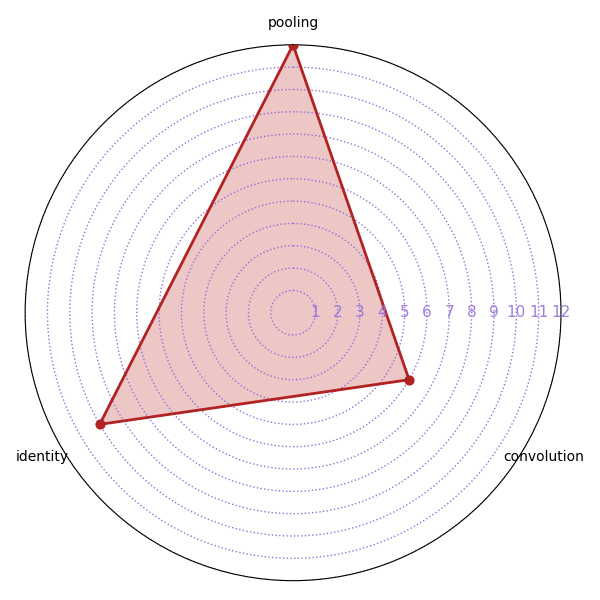
\includegraphics[width=\linewidth]{Figure_uniform.png}\\
        (A) равномерный штраф
    \end{minipage}\hfill
    \begin{minipage}[t]{0.48\linewidth}
        \centering
        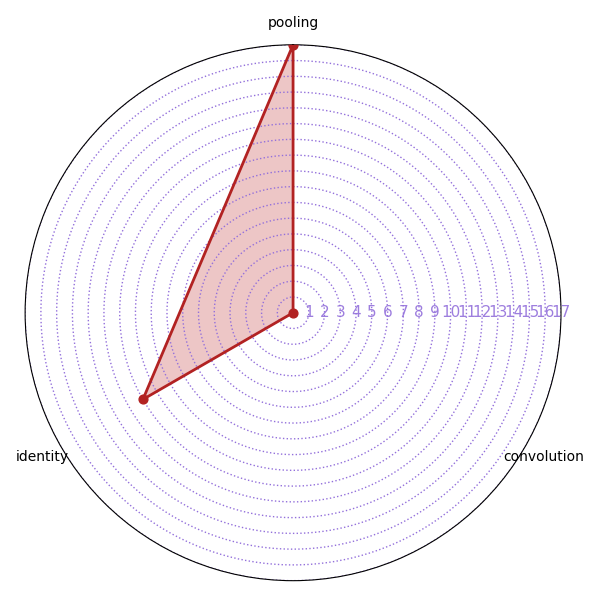
\includegraphics[width=\linewidth]{Figure_conv_penalty.png}\\
        (B) увеличенный за свёртки
    \end{minipage}

    \vspace{0.8em} % небольшое вертикальное расстояние между строками

    % --- 2-я строка ---
    \begin{minipage}[t]{0.48\linewidth}
        \centering
        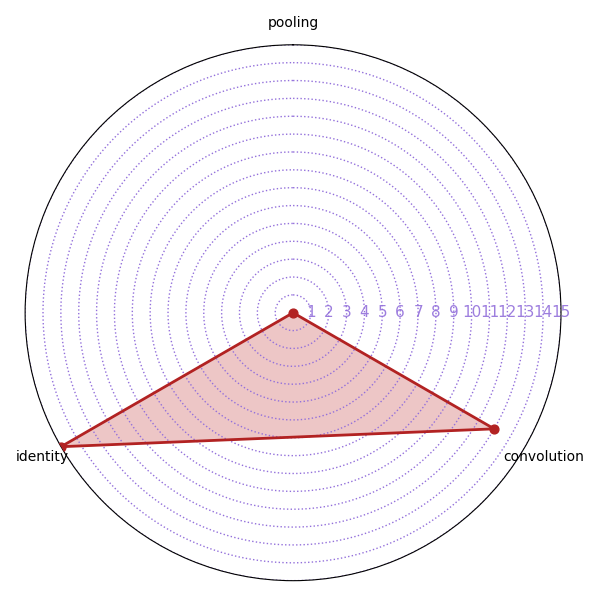
\includegraphics[width=\linewidth]{Figure_pool_penalty.png}\\
        (C) увеличенный за пулинг
    \end{minipage}\hfill
    \begin{minipage}[t]{0.48\linewidth}
        \centering
        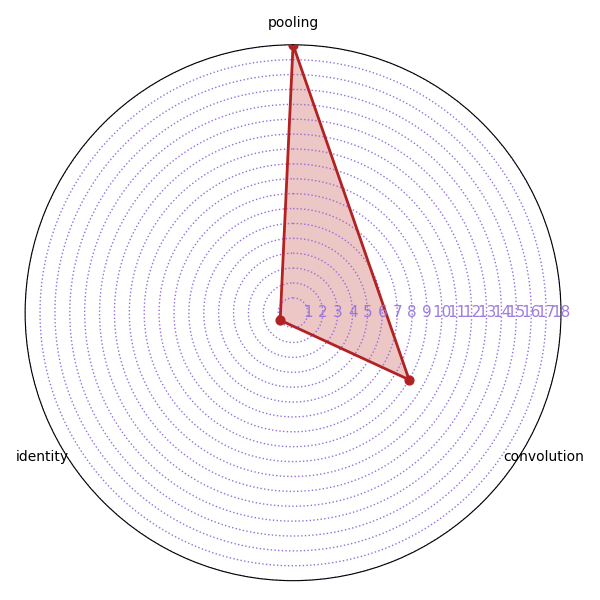
\includegraphics[width=\linewidth]{Figure_ident_penalty.png}\\
        (D) увеличенный за пропуск
    \end{minipage}

    \caption{Статистика по операциям для четырёх архитектур эксперимента 1: 
             \textbf{(A)} равномерный штраф, 
             \textbf{(B)} увеличенный за свёртки, 
             \textbf{(C)} увеличенный за пулинг, 
             \textbf{(D)} увеличенный за пропуск.}
    \label{fig2}
\end{figure}


\begin{table}[!ht]
    \centering
    
    \label{exp1}
    \begin{tabular}{lcccc}
        \hline
        & (A) uniform & (B) conv.\ penalty & (C) pool.\ penalty & (D) ident.\ penalty \\[2pt] \hline
        Test accuracy [\%]           & 82.5 & 79.2 & \textbf{85.0} & 81.4\\
        Parameter count              & 38\,304 & \textbf{5\,120} & \textbf{143\,488} &12\,320\\
        \# Pooling layers            & 12 & 17 & \textbf{0} & 18\\
        \# Convolution layers        & 6  & \textbf{0} & 13 & 9\\
        \# Identity connections      & 10 & 11 & 15 & \textbf{1} \\\hline
    \end{tabular}
    \caption{Сравнение количества слоёв в архитектурах эксперимента 1.}
\end{table}

\begin{table}[!ht]
    \centering
    \label{exp2}
    \begin{tabular}{lcccc}
        \hline
        & (A) uniform & (B) conv.\ penalty  & (C) pool.\ penalty & (D) ident.\ penalty \\[2pt] \hline
        Test accuracy [\%] & 85.62 & 82.37  & \textbf{85.63} & 85.60 \\
        Parameter count          & 93\,888 & \textbf{25\,280}  & \textbf{137\,632} & 72\,928\\
        \# Pooling layers & 16 & 22  & \textbf{4} & 22\\
        \# Convolution layers & 8 & \textbf{1}  & 13 & 6 \\
        \# Identity connections         & 4 & 5  & 11 & \textbf{0}\\ \hline
    \end{tabular}
    \caption{Сравнение количества слоёв в архитектурах эксперимента 2.}
\end{table}

\begin{table}[!ht]
    \centering
    \label{exp3}
    \begin{tabular}{lcccc}
        \hline
        & (A) uniform & (B) conv.\ penalty  & (C) pool.\ penalty & (D) ident.\ penalty \\[2pt] \hline
        Test accuracy [\%] & 71.02 & 52.37  & \textbf{73.77} & 68.43 \\
        Parameter count   & 113\,984 &10\,240  & \textbf{159\,456} & \textbf{8\,800}\\
        \# Pooling layers & 4 & 12  & \textbf{0} & 17\\
        \# Convolution layers & 18 & \textbf{0}  & 9 & 11 \\
        \# Identity connections & 6 & 16  & 19 & \textbf{0}\\ \hline
    \end{tabular}
    \caption{Сравнение количества слоёв в архитектурах эксперимента 3.}
\end{table}

\newpage
Результаты экспериментов показывают, что при равномерном штрафе используются все операции и получается среднее, среди рассмотренных вариантов, качество и количество параметров. При увеличенном штрафе за свёртки падает качество модели и минимизируется использование соответствующих операций, при этом количество параметров уменьшается, что можно использовать при соответствующих эксплуатационных ограничениях. При увеличенном штрафе за пулинг уменьшается количество операций пулинга. За счёт этого возрастает количество свёрток и соответственно увеличивается количество параметров, а также получается наилучшее качество. При увеличенном штрафе за пропуск исчезают операции identity.

Общие выводы по экспериментам:

\begin{itemize}

\item \textbf{Контроль операций}. Результаты экспериментов подтверждают возможность гибкого контроля над типами операций: при использовании вектора сложности с увеличенным штрафом за операцию --- она перестаёт использоваться в модели. 
\item \textbf{Управляемая сложность.} Метод позволяет изменяя вектор $\boldsymbol{s}$ перемещаться вдоль парето-фронта точность-сложность, получая модели с количеством параметров от 5 до 150 тысяч.
\item \textbf{Эксплуатационные ограничения.} Проассоциировав операции со временем их выполнения на устройстве, метод позволяет подобрать архитектуру для уменьшения ожидаемого времени выполнения модели на целевом устройстве, за счёт уменьшения количества долго выполняющихся операций. Аналогично можно поступить при необходимости минимизировать не время, а энергетические затраты или любые другие эксплуатационные ограничения.
\item \textbf{Семейство моделей.} Все рассматриваемые варианты внутри каждого отдельного эксперимента порождены одной обученной моделью, таким образом метод представляет целое семейство готовых моделей и механизм гибкого выбора из него.
\item \textbf{Согласованность результатов.} Все рассмотренные зависимости сохраняются на разных наборах и списках операций, что подтверждает универсальность метода.

\end{itemize}


\section{Заключение}

Предложен метод для выбора архитектуры модели глубокого обучения с контролем характеристик на целевом устройстве сочетающий точность модели и эффективность  аппаратного исполнения. Преимущества метода в том, что за один процесс обучения порождается семейство архитектур, а введённый вектор сложности позволяет интуитивно контролировать операции при выборе моделей. Такой подход позволяет получать модели под конкретные аппаратные ограничения без дополнительного обучения под эти требования. В экспериментальной части подтверждена работоспособность метода на разных наборах данных и при различных наборах допустимых операций.  


В рамках дальнейшего развития метода планируется добавление многокритериального учета сложности и проведение полноформатного сопоставления результатов с классическими NAS-подходами.

% теорема

\bibliographystyle{plain}
\bibliography{sample}

\end{document}